%%%%%%%%%%%%%%%%%%%%%%%%%%%%%%%%%%%%%%%%%%%%%%%%%%%%%%%%%%%%%%%
%
% Welcome to Overleaf --- just edit your LaTeX on the left,
% and we'll compile it for you on the right. If you open the
% 'Share' menu, you can invite other users to edit at the same
% time. See www.overleaf.com/learn for more info. Enjoy!
%
%%%%%%%%%%%%%%%%%%%%%%%%%%%%%%%%%%%%%%%%%%%%%%%%%%%%%%%%%%%%%%%
\documentclass{beamer}
\usepackage{babel,blindtext}
\usepackage[backend=biber,isbn=false,url=false]{biblatex} 
\usepackage{caption}
\setbeamerfont{caption}{size=\scriptsize} 
\addbibresource{refsPres.bib}
\setbeamerfont{footnote}{size=\tiny}
\usetheme{Berlin}
%Information to be included in the title page:
\title{Algorithmic Transit Optimization: Evolutionary Algorithms Applied}
\author{Harrison Weinstock}
\institute{Haverford College}
\date{\today}

\begin{document}

\frame{\titlepage}

\section{Background Info}
\begin{frame}{Designing a System}

\minipage{0.33\textwidth}
  \begin{enumerate}
    \item \textbf{Network geometry}
    \item Frequency Assignment and Timetable Development
    \item Fleet and Crew Scheduling
    \end{enumerate}
\endminipage\hfill
\minipage{0.66\textwidth}%
\begin{figure}
  \fbox{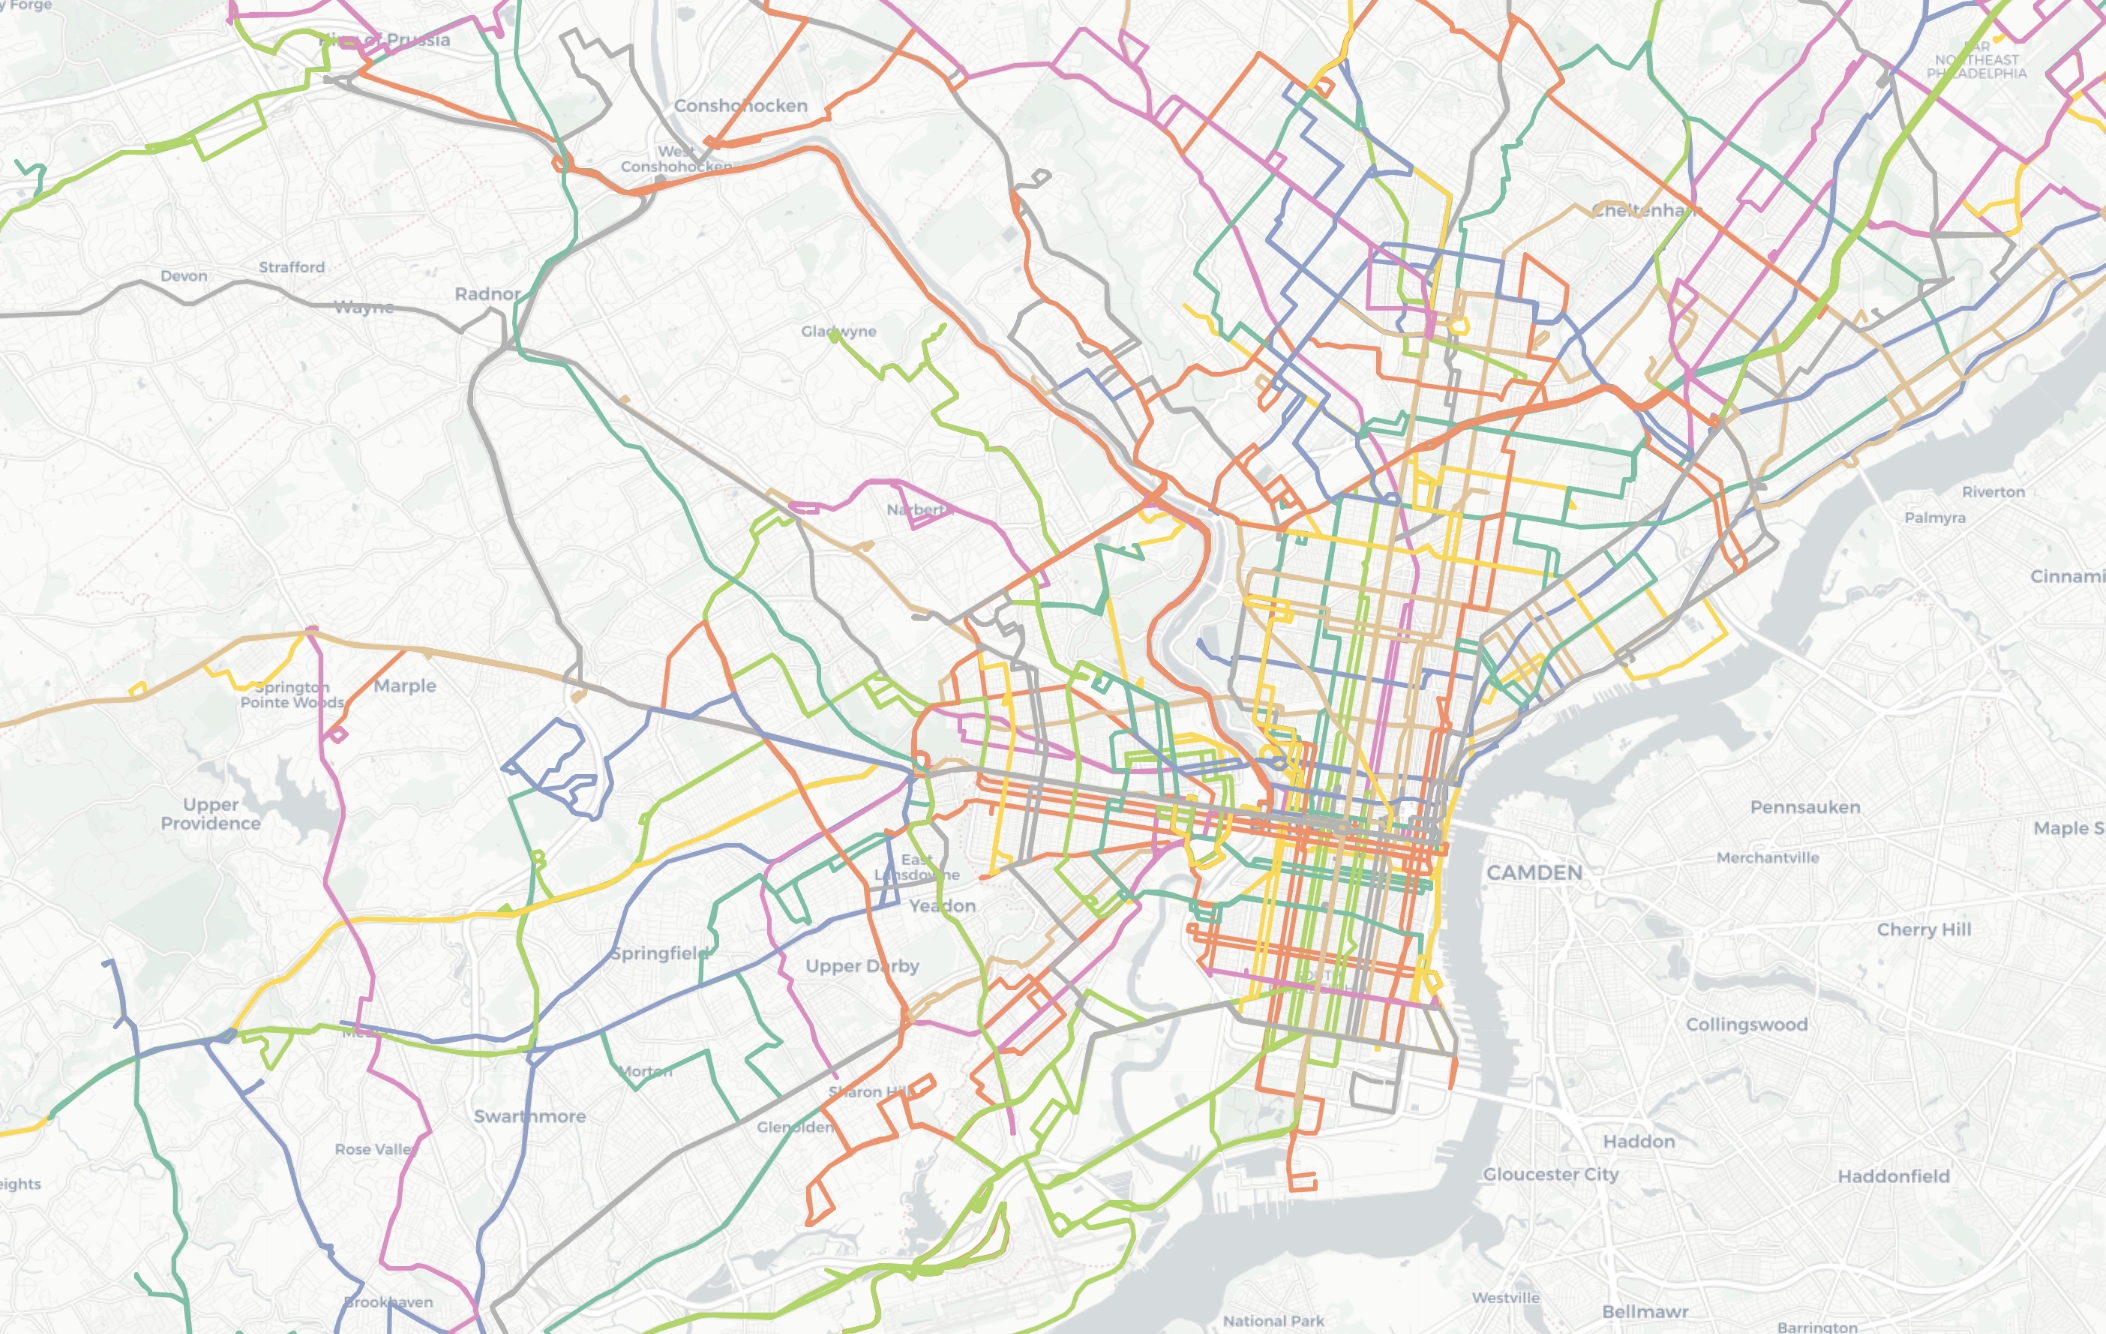
\includegraphics[width=\linewidth]{Presentation/diagrams/septa_screenshot.png}}
  \caption{SEPTA Service around Philadelphia \cite{SEPTA}}
\end{figure}
\endminipage
\end{frame}

\begin{frame}
\frametitle{Urban Public Transit Optimization}
\begin{figure}[!htb]
\minipage{0.42\textwidth}
  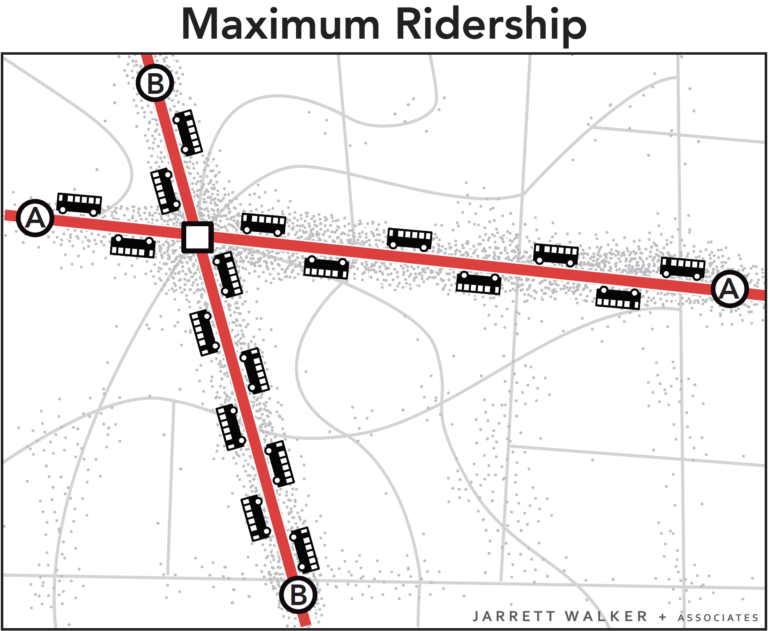
\includegraphics[width=\linewidth]{Presentation/diagrams/covVersusRide_2.png}
  \caption{Optimizing for Ridership \cite{walker2012}}\label{fig:ridership}
\endminipage\hfill
\minipage{0.42\textwidth}%
  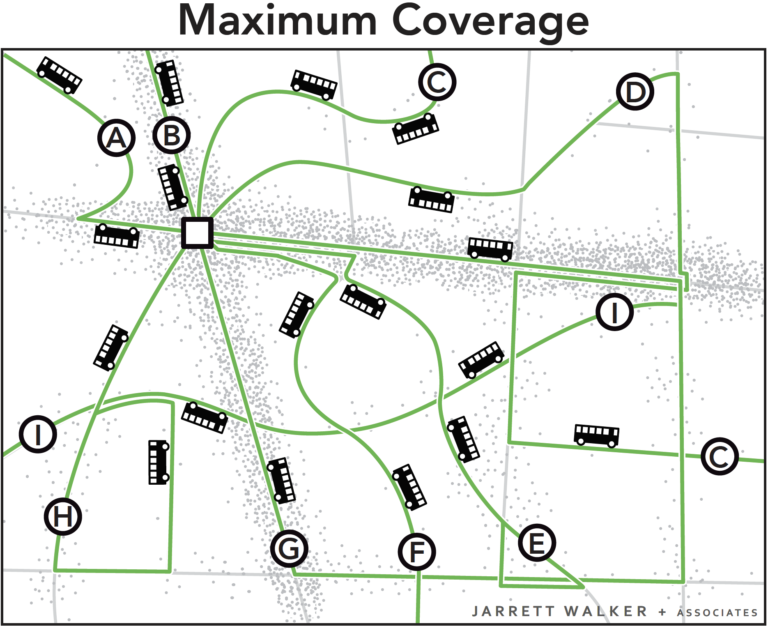
\includegraphics[width=\linewidth]{Presentation/diagrams/covVersusRide_3.png}
  \caption{Optimizing for Coverage \cite{walker2012}}\label{fig:coverage}
\endminipage
\end{figure}
\textbf{Other examples of trade-offs:}
\begin{enumerate}
    \item \textit{User Costs} versus \textit{Operator Costs}.  
    \item \textit{Network Simplicity} versus \textit{Functionality}. 
    \item \textit{Direct} versus \textit{Frequency}. 
\end{enumerate}
\end{frame}

\begin{frame}{Genetic Algorithms}
    \begin{center}
    \fbox{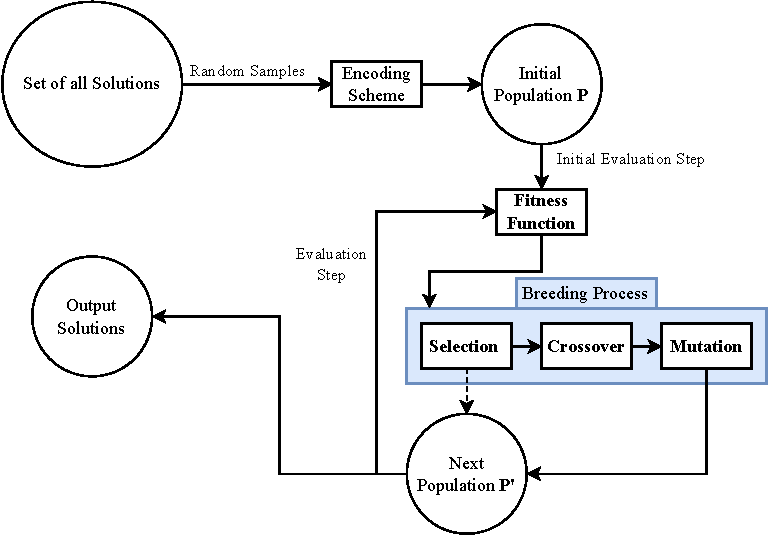
\includegraphics[width=0.8\linewidth]{Presentation/diagrams/general_ga.pdf}}
    \end{center}
\end{frame}

\section{The Model}

\begin{frame}{Outline of Custom GA}
    \fbox{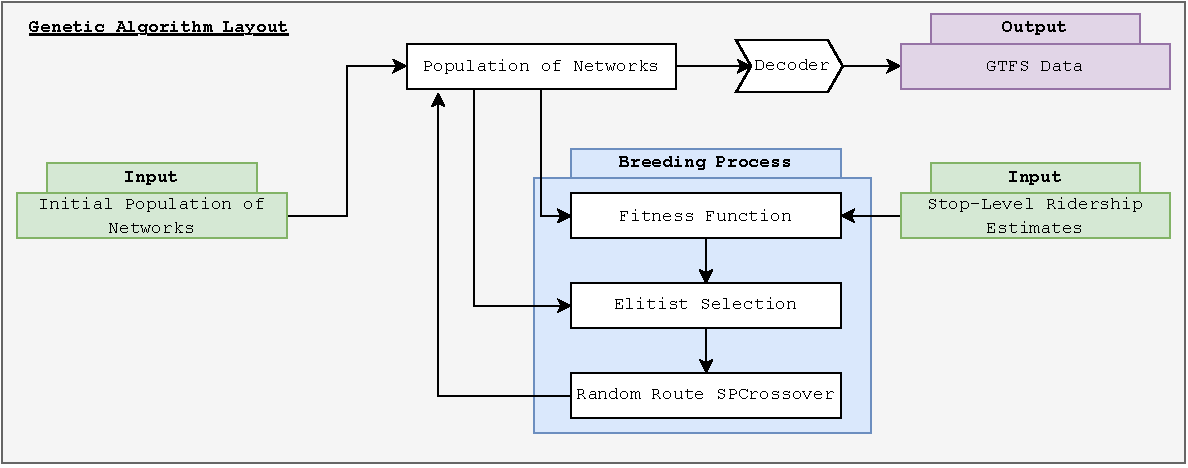
\includegraphics[width=\linewidth]{Presentation/diagrams/GeneticAlgorithmPlan.pdf}}
\end{frame}

\begin{frame}{SPCrossover: The Crossover Operation}
\begin{figure}
\minipage{0.49\textwidth}
  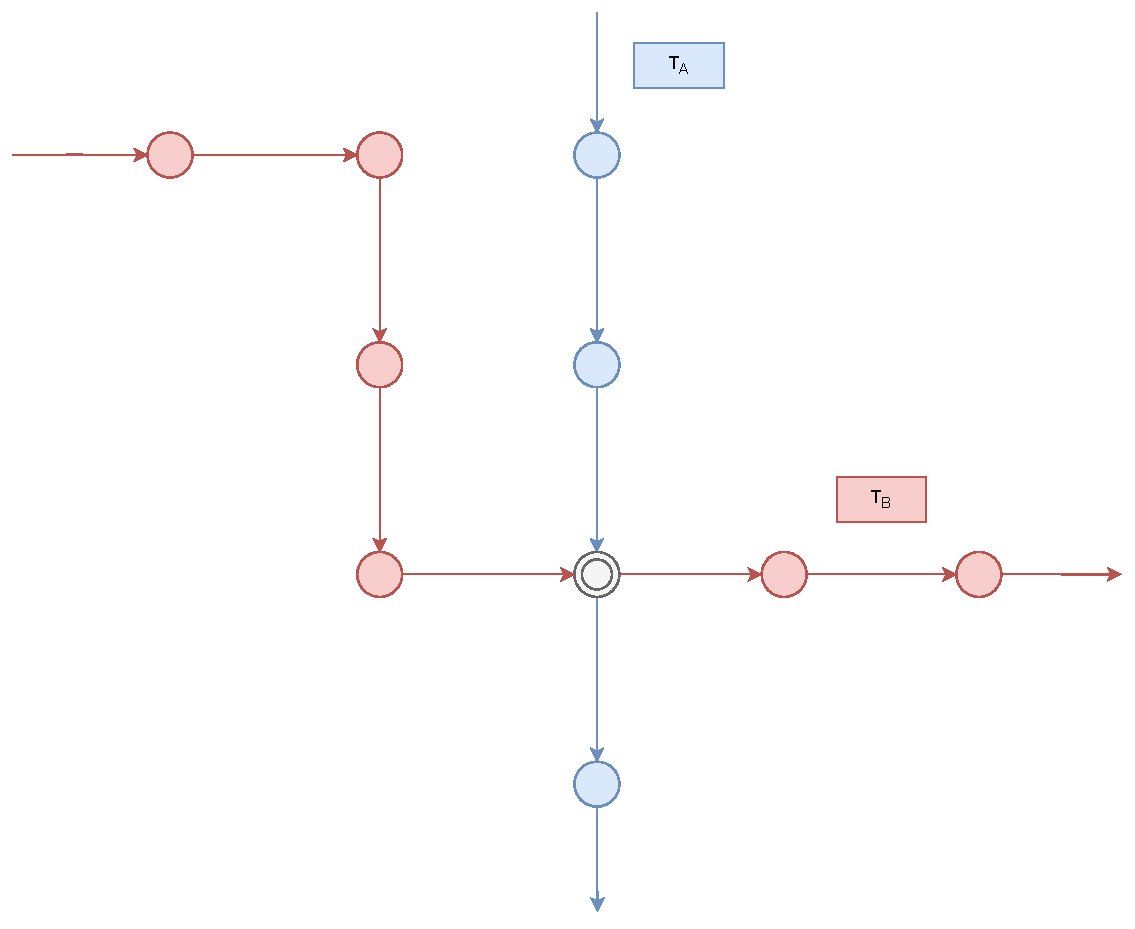
\includegraphics[width=\linewidth]{Presentation/diagrams/route-crossover1.pdf}
  \caption{Original 'parent' routes}\label{fig:parents}
\endminipage\hfill
\minipage{0.49\textwidth}%
  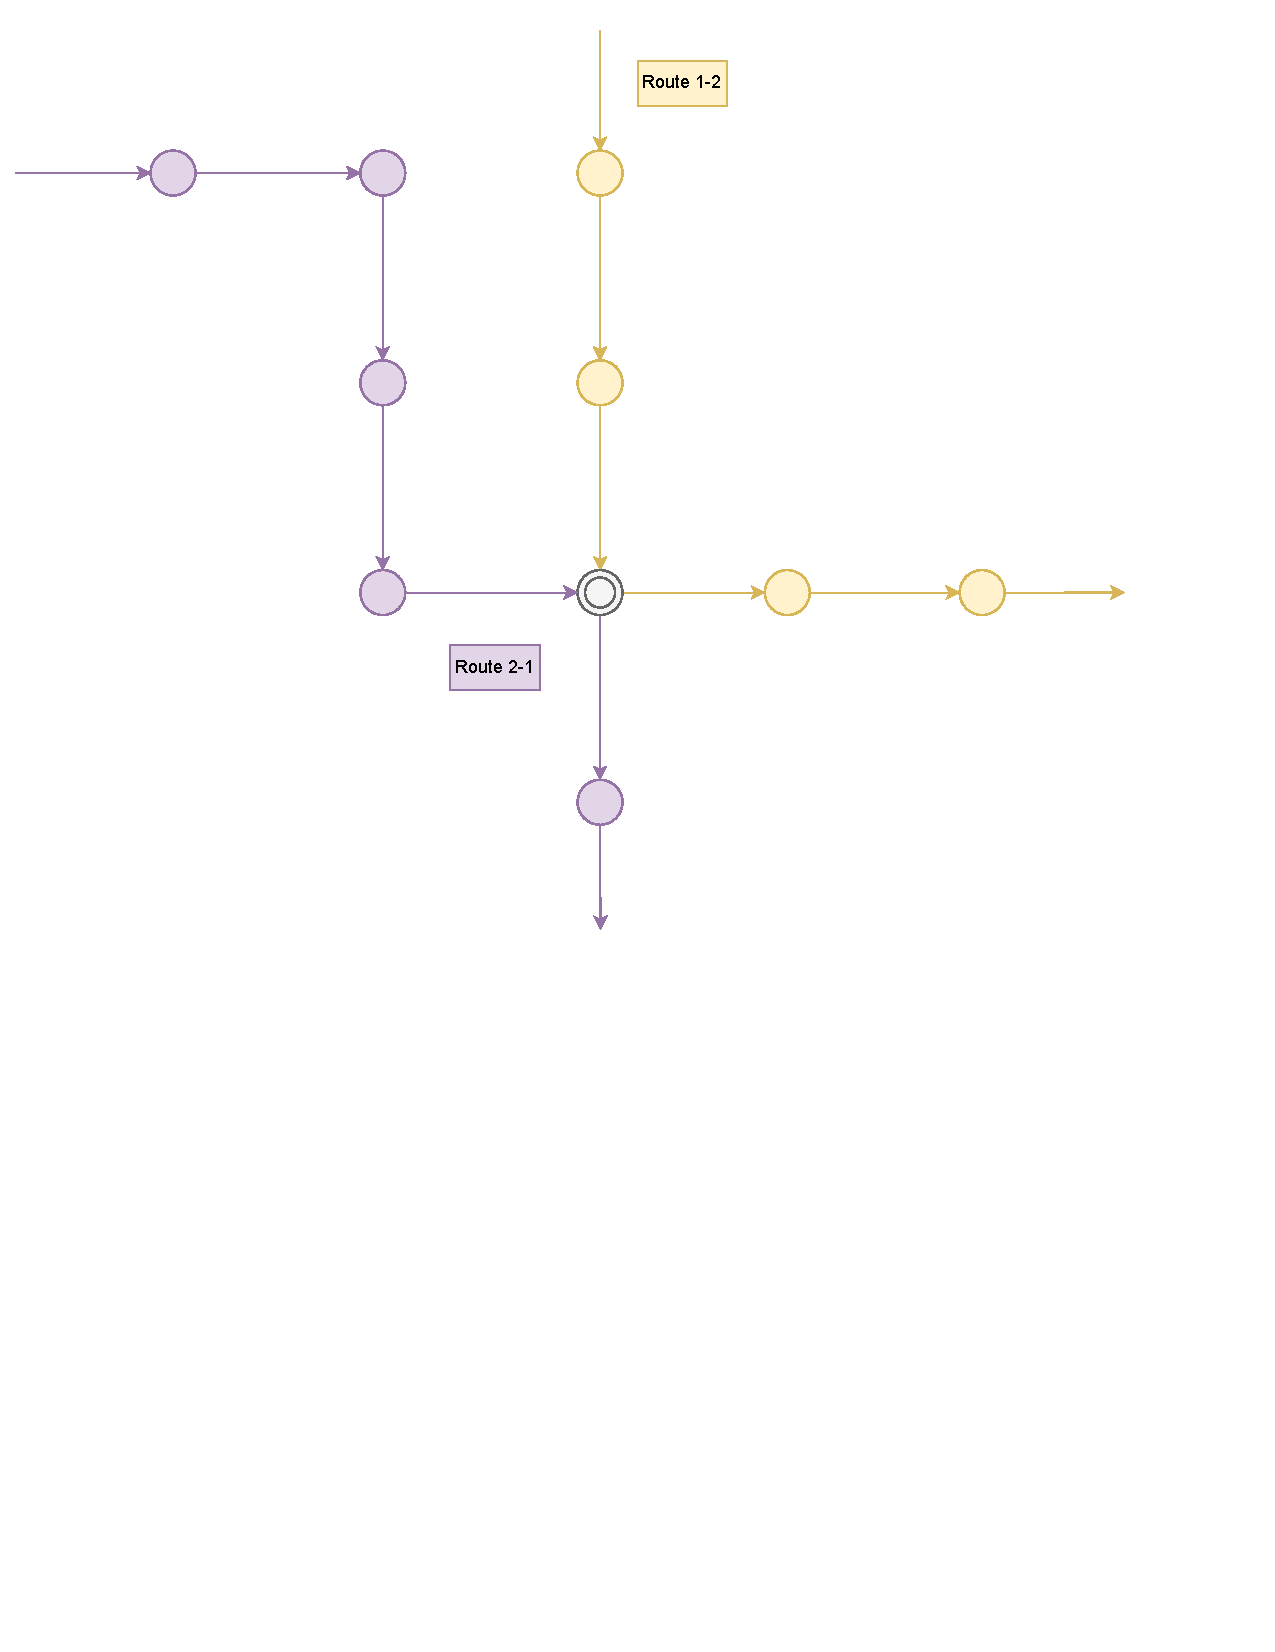
\includegraphics[width=\linewidth]{Presentation/diagrams/route-crossover2.pdf}
  \caption{New 'children' routes}\label{fig:children}
\endminipage
\begin{itemize}
    \item Focus on \textbf{transfer points} as crossover points. 
    \item Work with \textbf{simple routes} where only transfer points are considered. 
\end{itemize}
\end{figure}
\end{frame}

\section{Implementation}
\begin{frame}{First step: Processing Data}
    \fbox{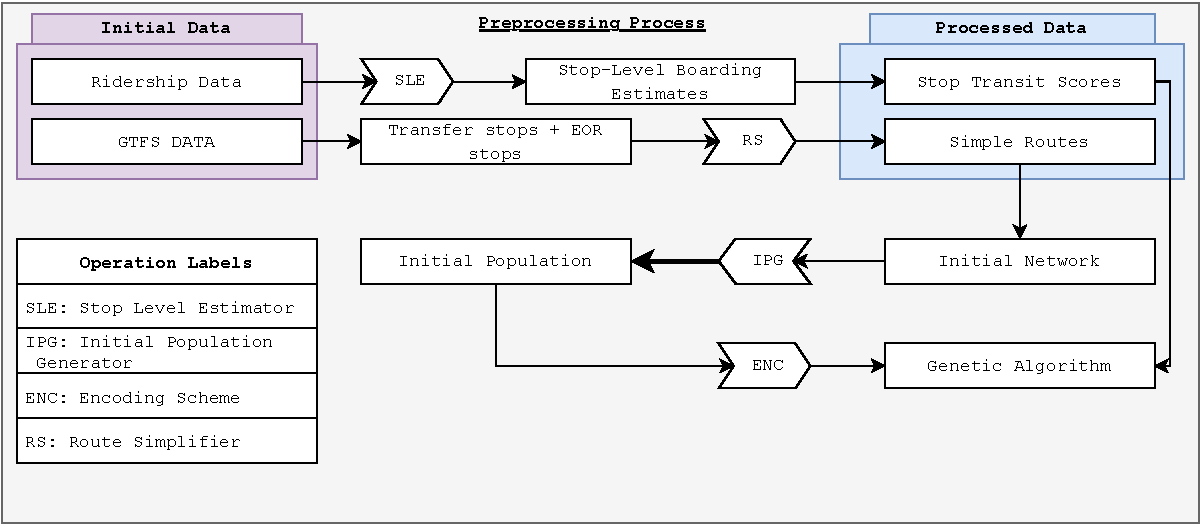
\includegraphics[width=\linewidth]{Presentation/diagrams/preprocessing_steps.pdf}}
    \begin{itemize}
        \item \textbf{Ridership Data:} Average total ridership by month by route. 
        \item \textbf{GTFS Data:} General Transit Feed Specification. 
    \end{itemize}
\end{frame}

\begin{frame}{Route Simplification}
    \begin{figure}[!htb]
\minipage{0.35\textwidth}
  \frame{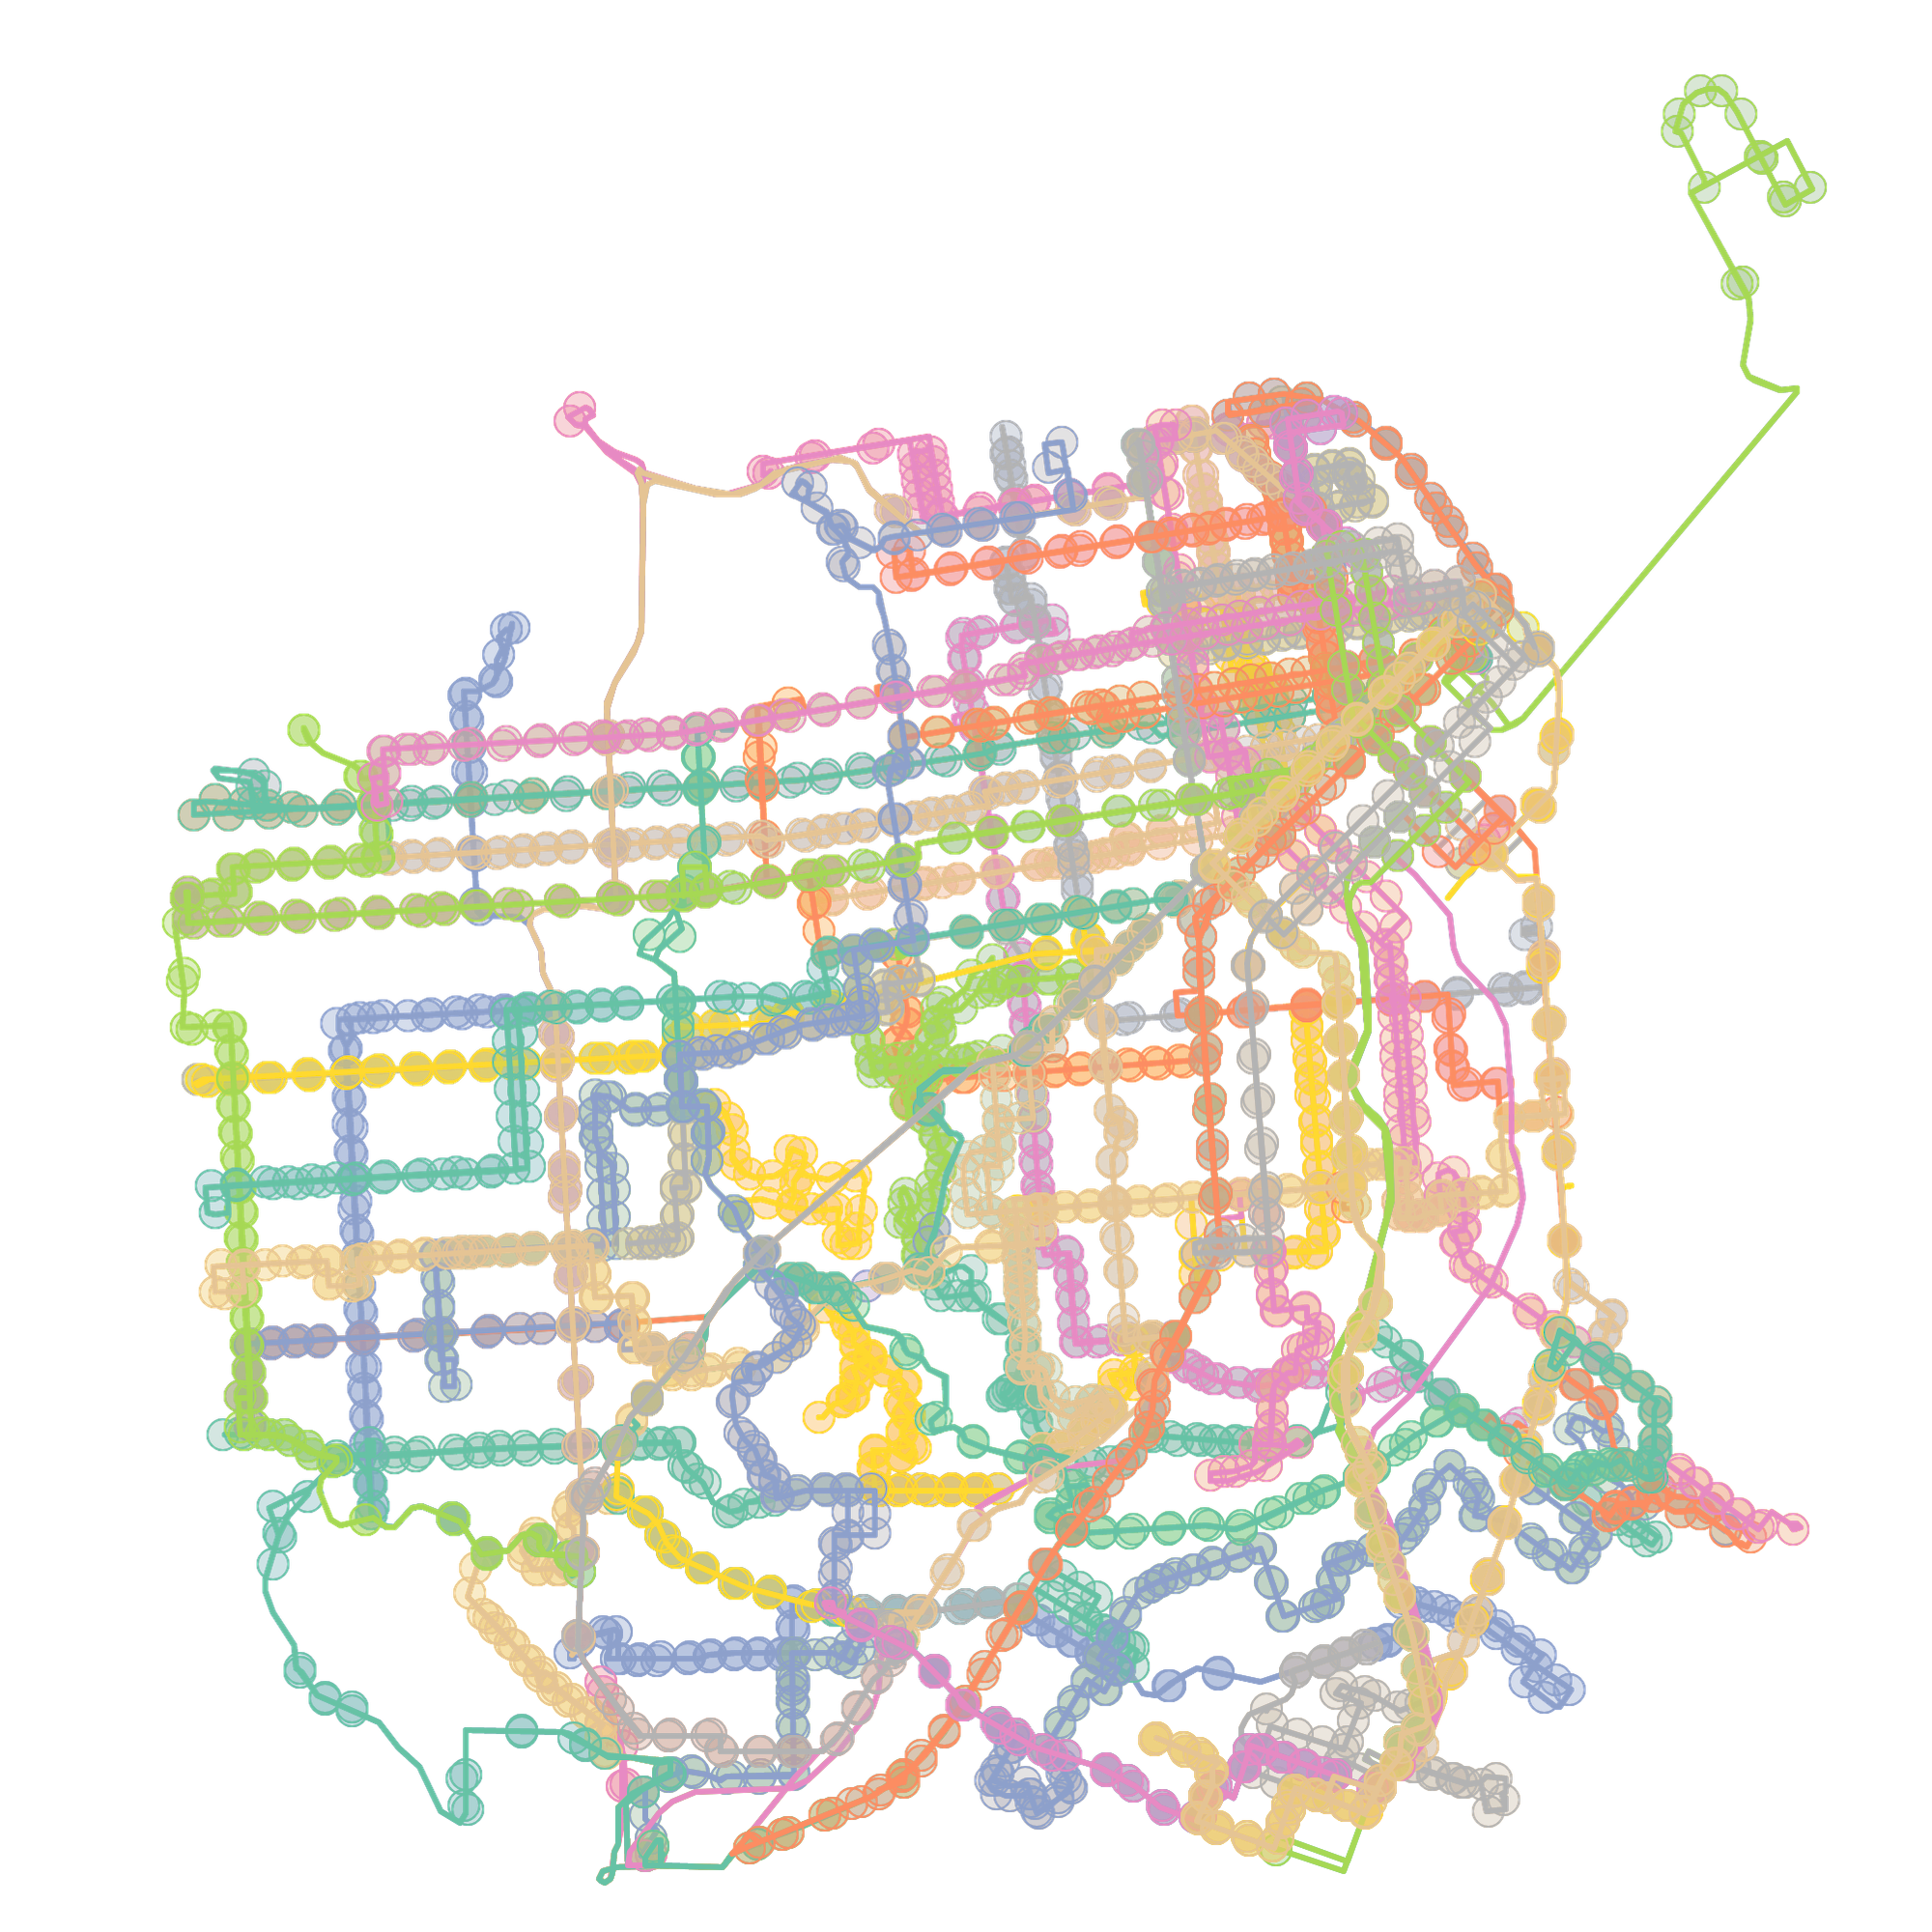
\includegraphics[width=\linewidth]{Presentation/diagrams/original_network.png}}
  \caption{Original Network}\label{fig:original-network}
\endminipage
\minipage{0.35\textwidth}%
  \frame{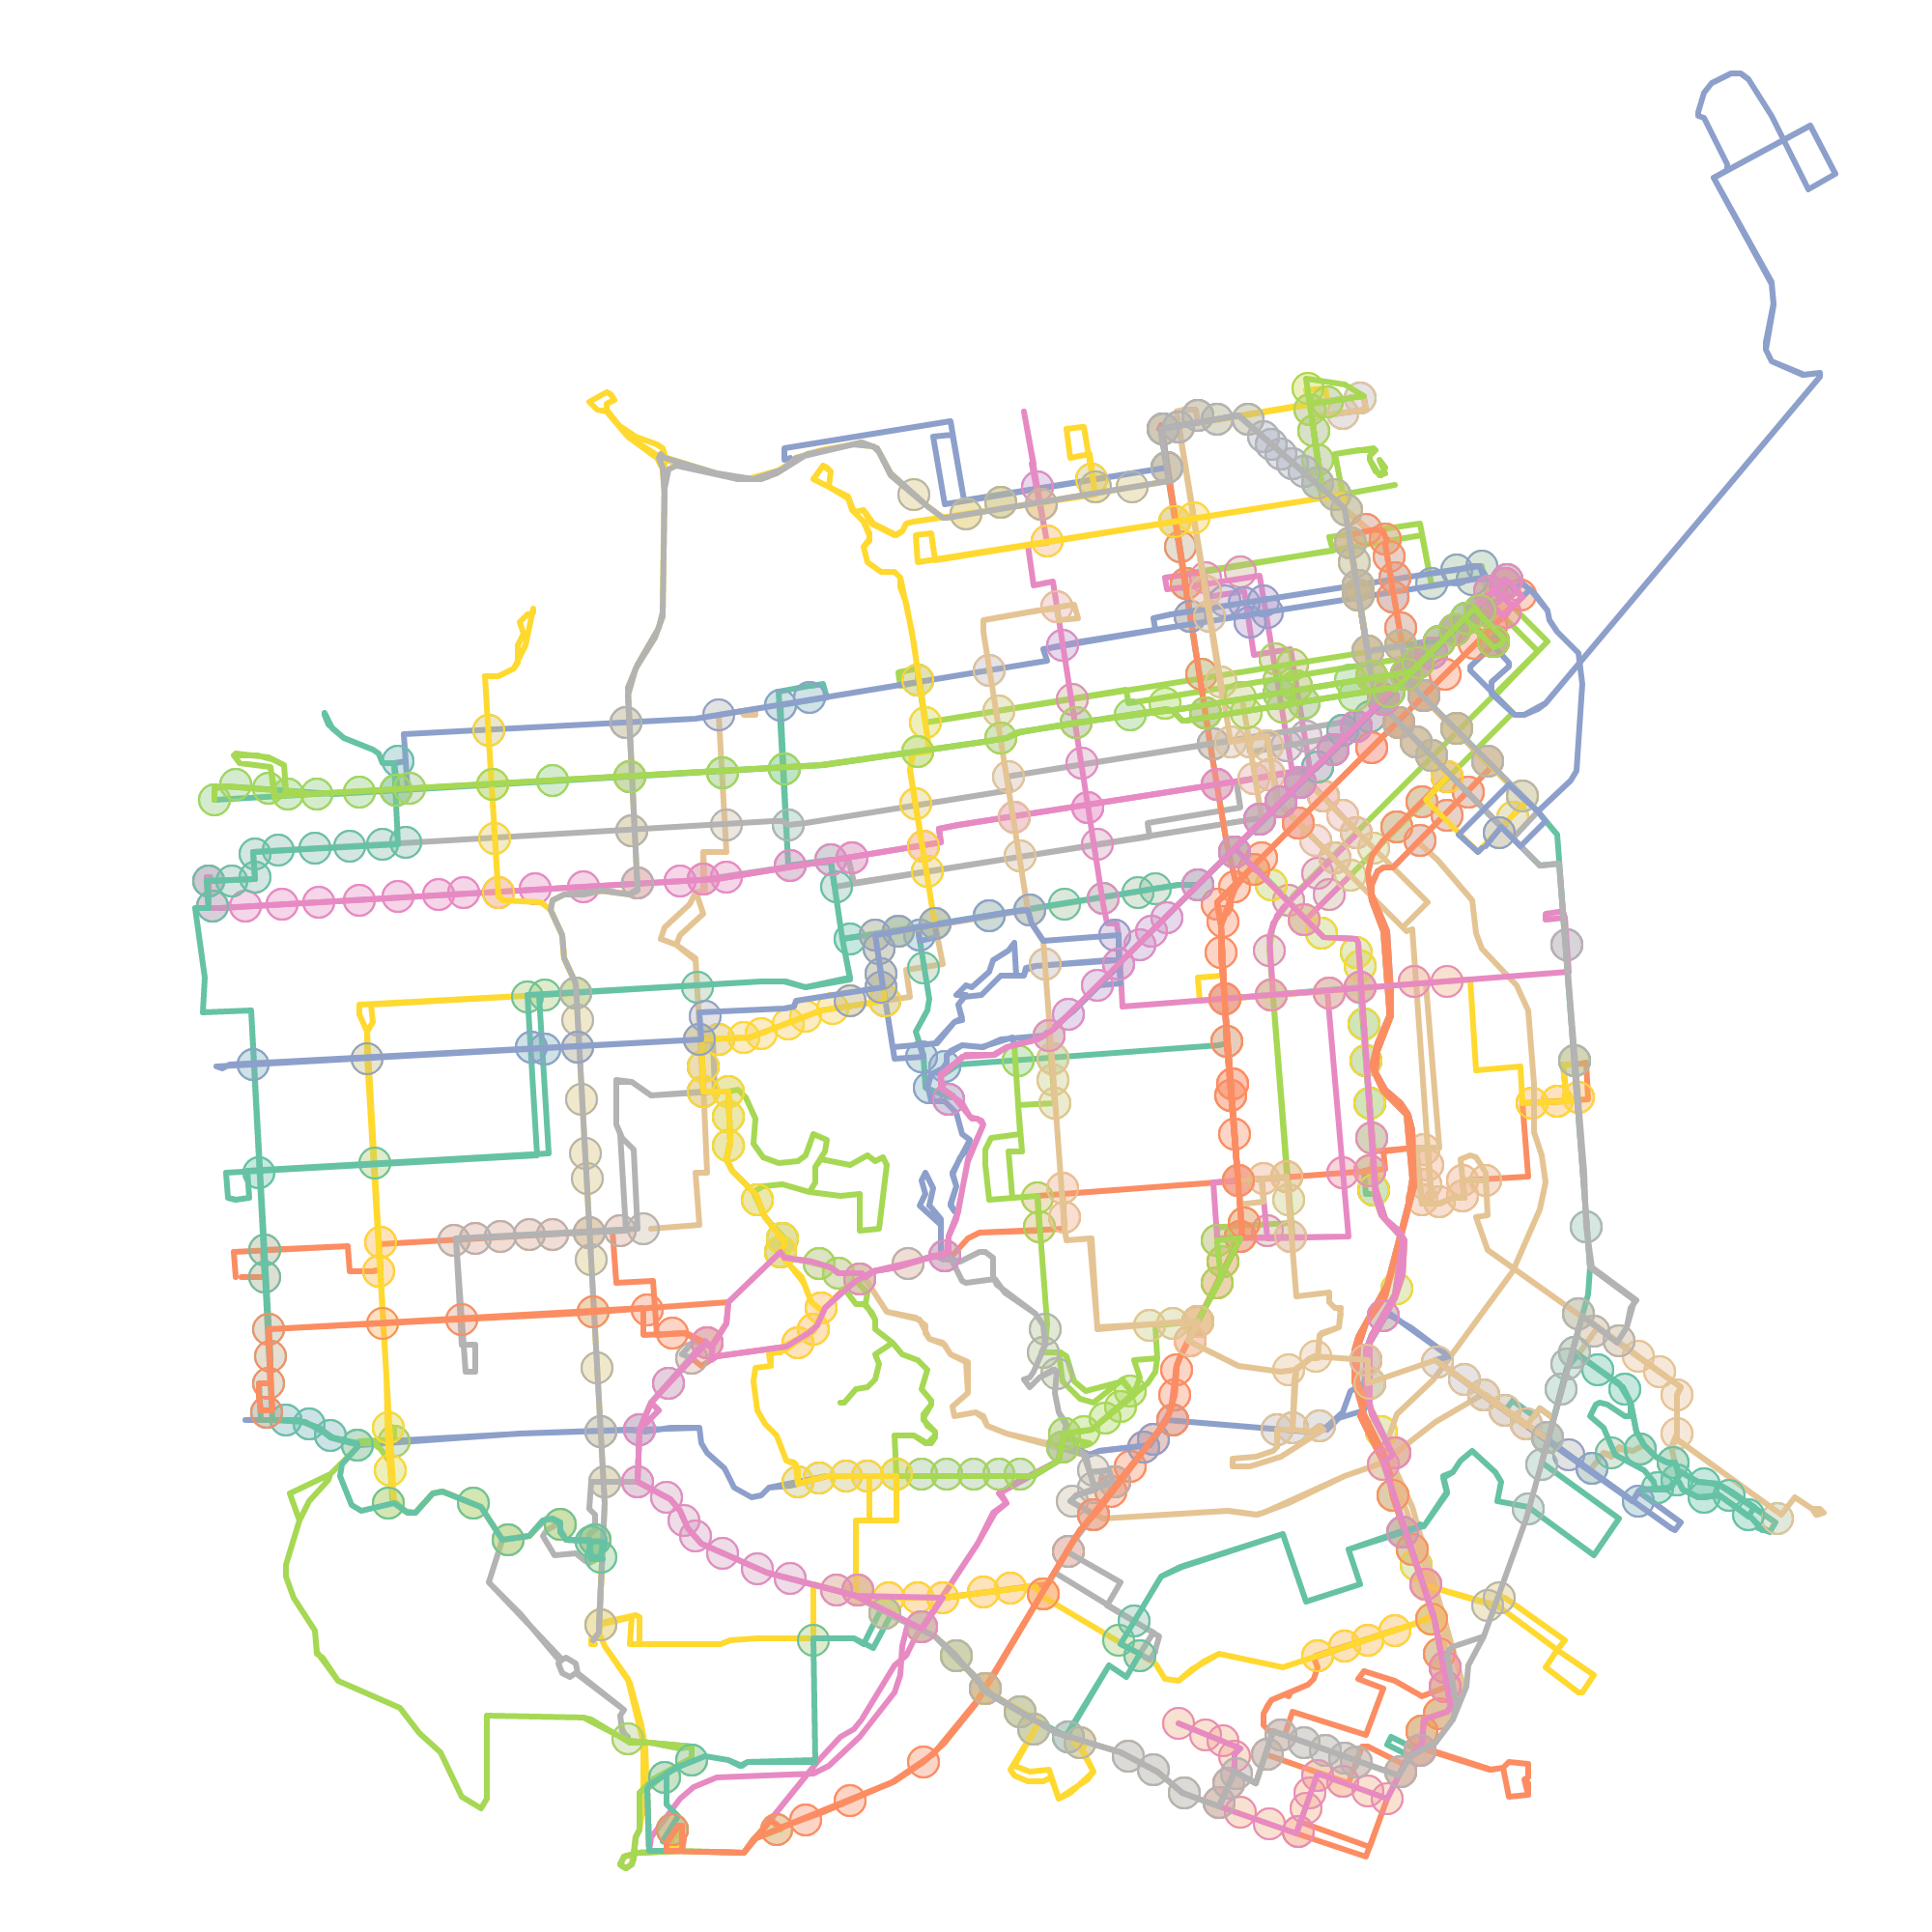
\includegraphics[width=\linewidth]{Presentation/diagrams/simplified_network.png}}
  \caption{Simplified Network}\label{fig:simplified-network}
\endminipage
\end{figure}
\begin{itemize}
        \item Reduced number of routes by over $50\%$. 
        \item Trips from about 50,000 to 106. 
        \item Stops by over $80\%$.
    \end{itemize}
\end{frame}


\section{Initial Version}
\begin{frame}{Fitness Function}
    \begin{center}
    \fbox{ 
    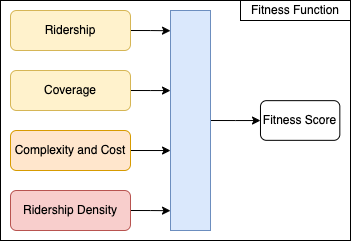
\includegraphics[width=0.5\linewidth]{Presentation/diagrams/initial-fitness-function.png}}
    \end{center}
    \begin{itemize}
        \item \textbf{4 keys factors.} 
        \item \textbf{Linear Combination} of factors based on experimental hyper-parameters. 
    \end{itemize}
\end{frame}

\begin{frame}{Results}
\begin{figure}
\frame{
\minipage{0.33\textwidth}
  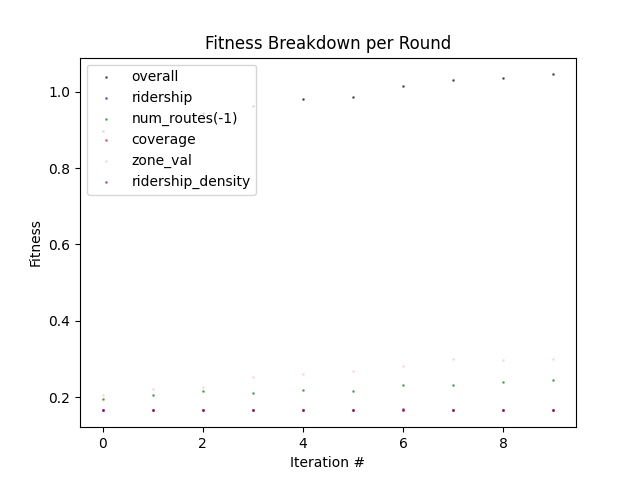
\includegraphics[width=\linewidth]{Presentation/diagrams/fitness_breakdown.png}
  \caption{Fitness per round}\label{fig:fitness_breakdown}
\endminipage
\minipage{0.33\textwidth}
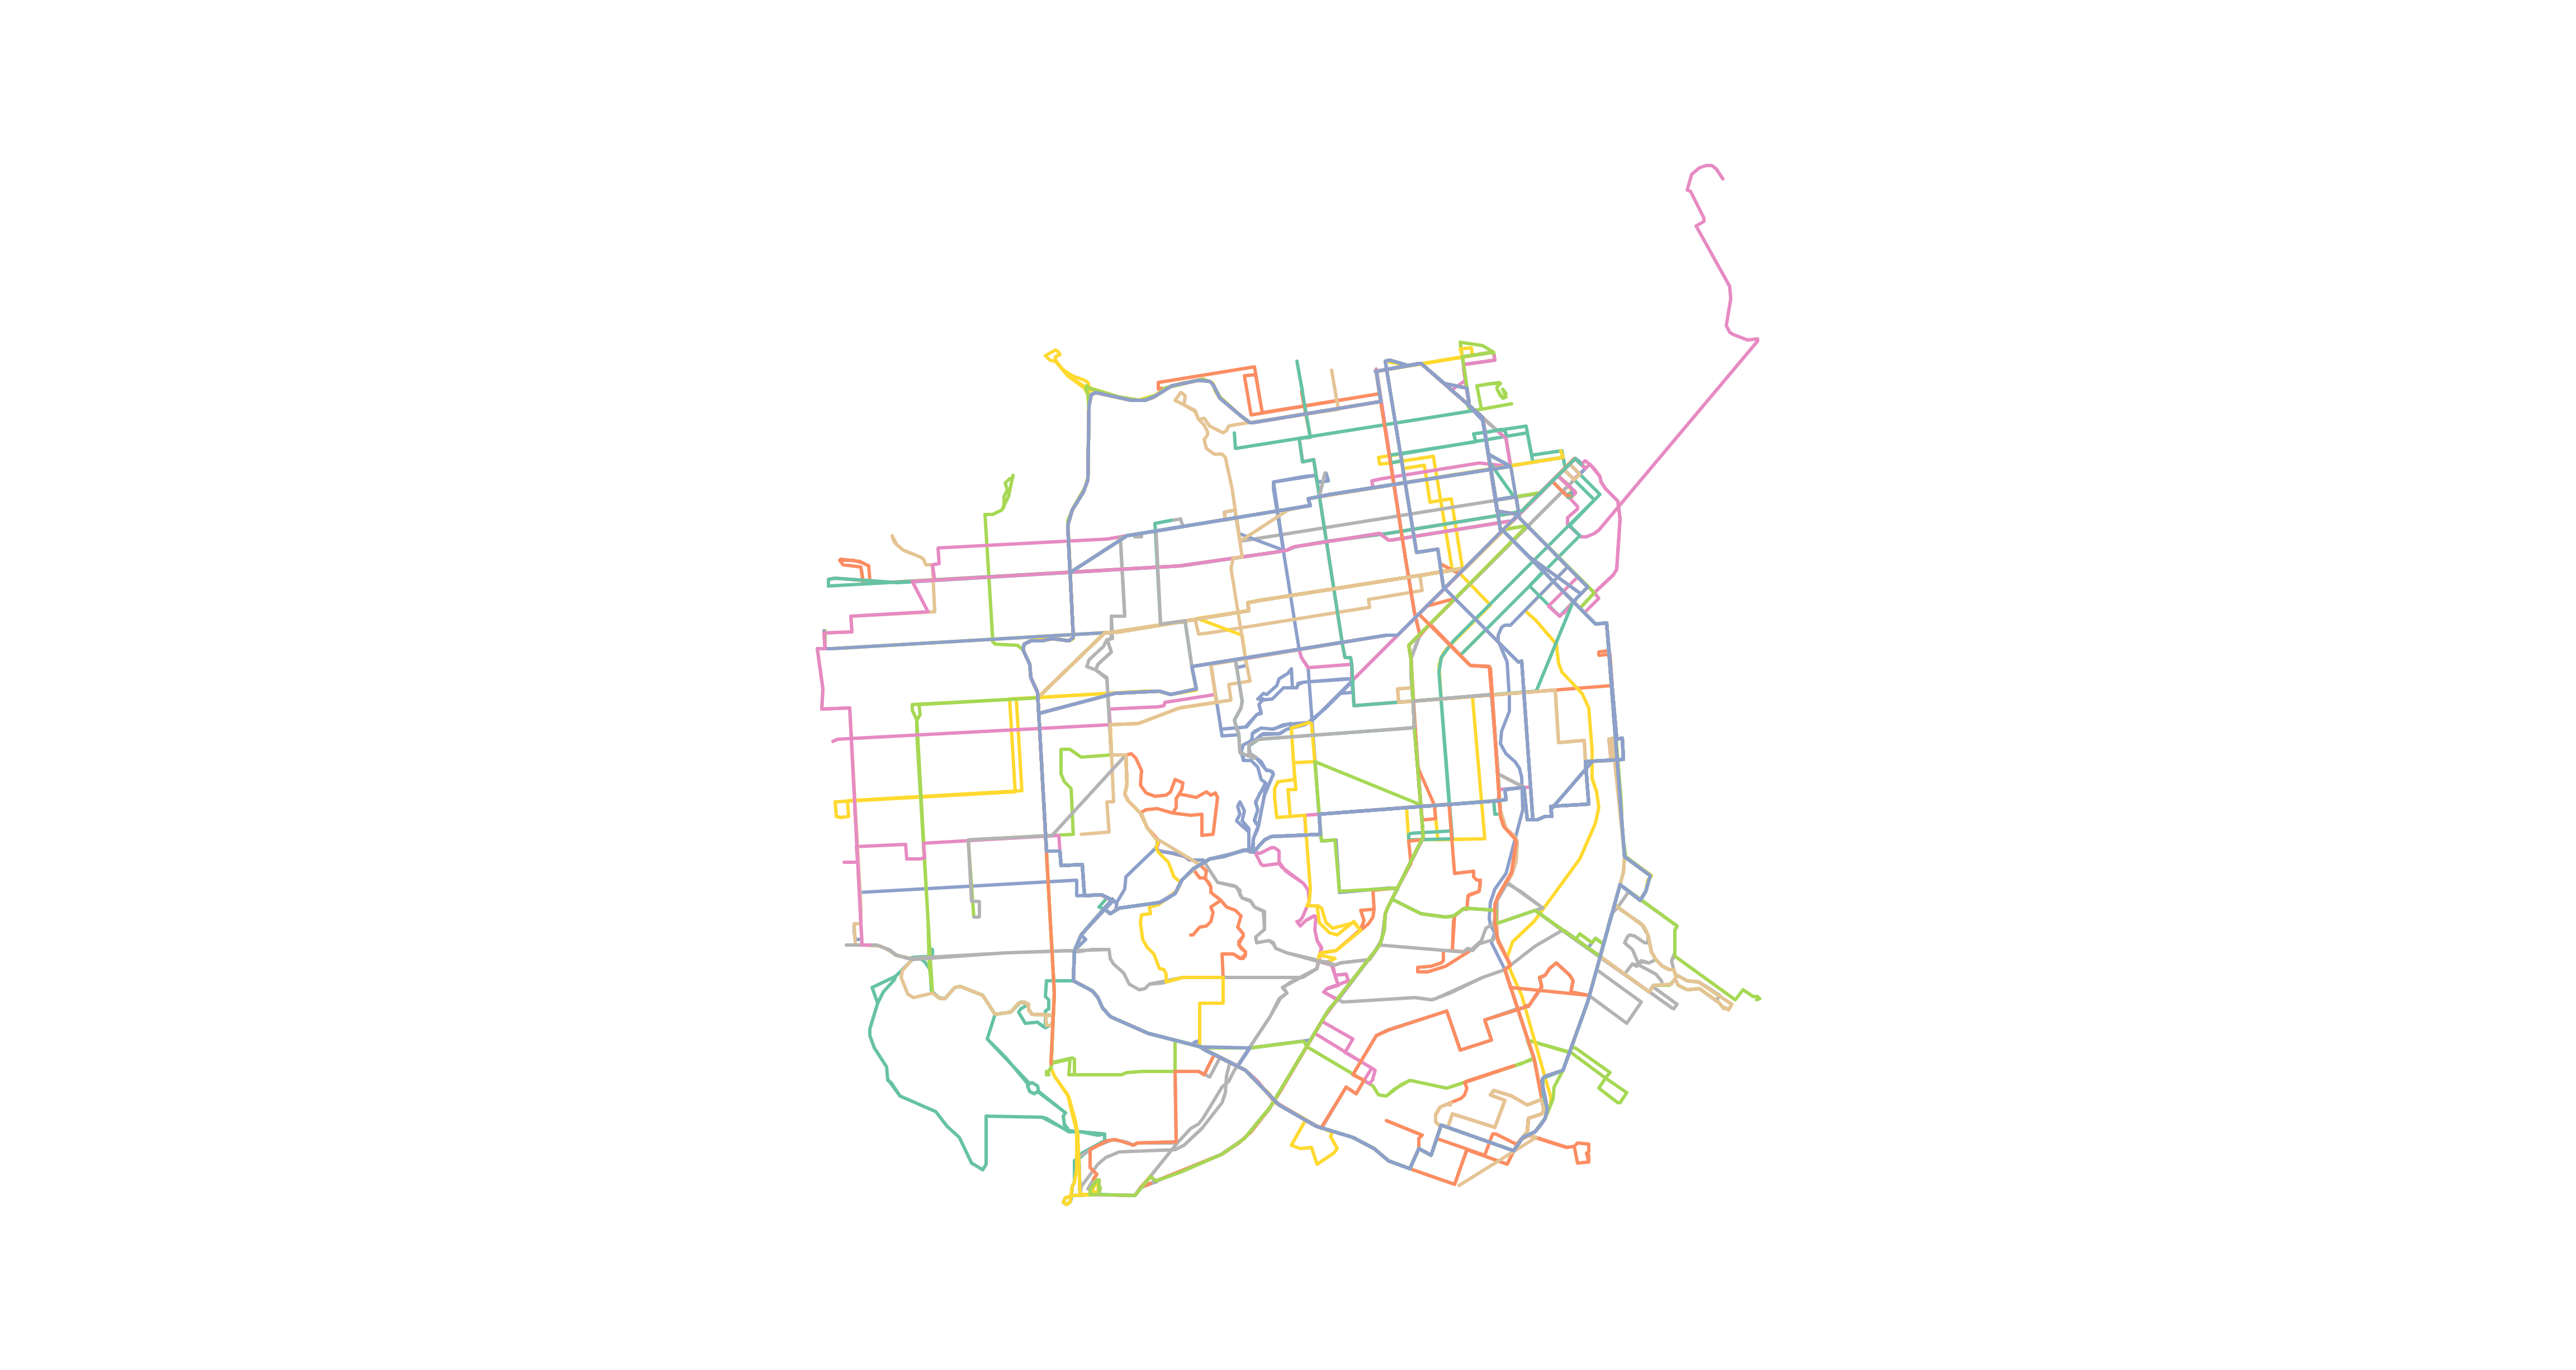
\includegraphics[width=\linewidth]{Thesis/diagrams/first_run/best_performer.png}
  \caption{Best Performer}\label{fig:long_route}
\endminipage
\minipage{0.33\textwidth}%
  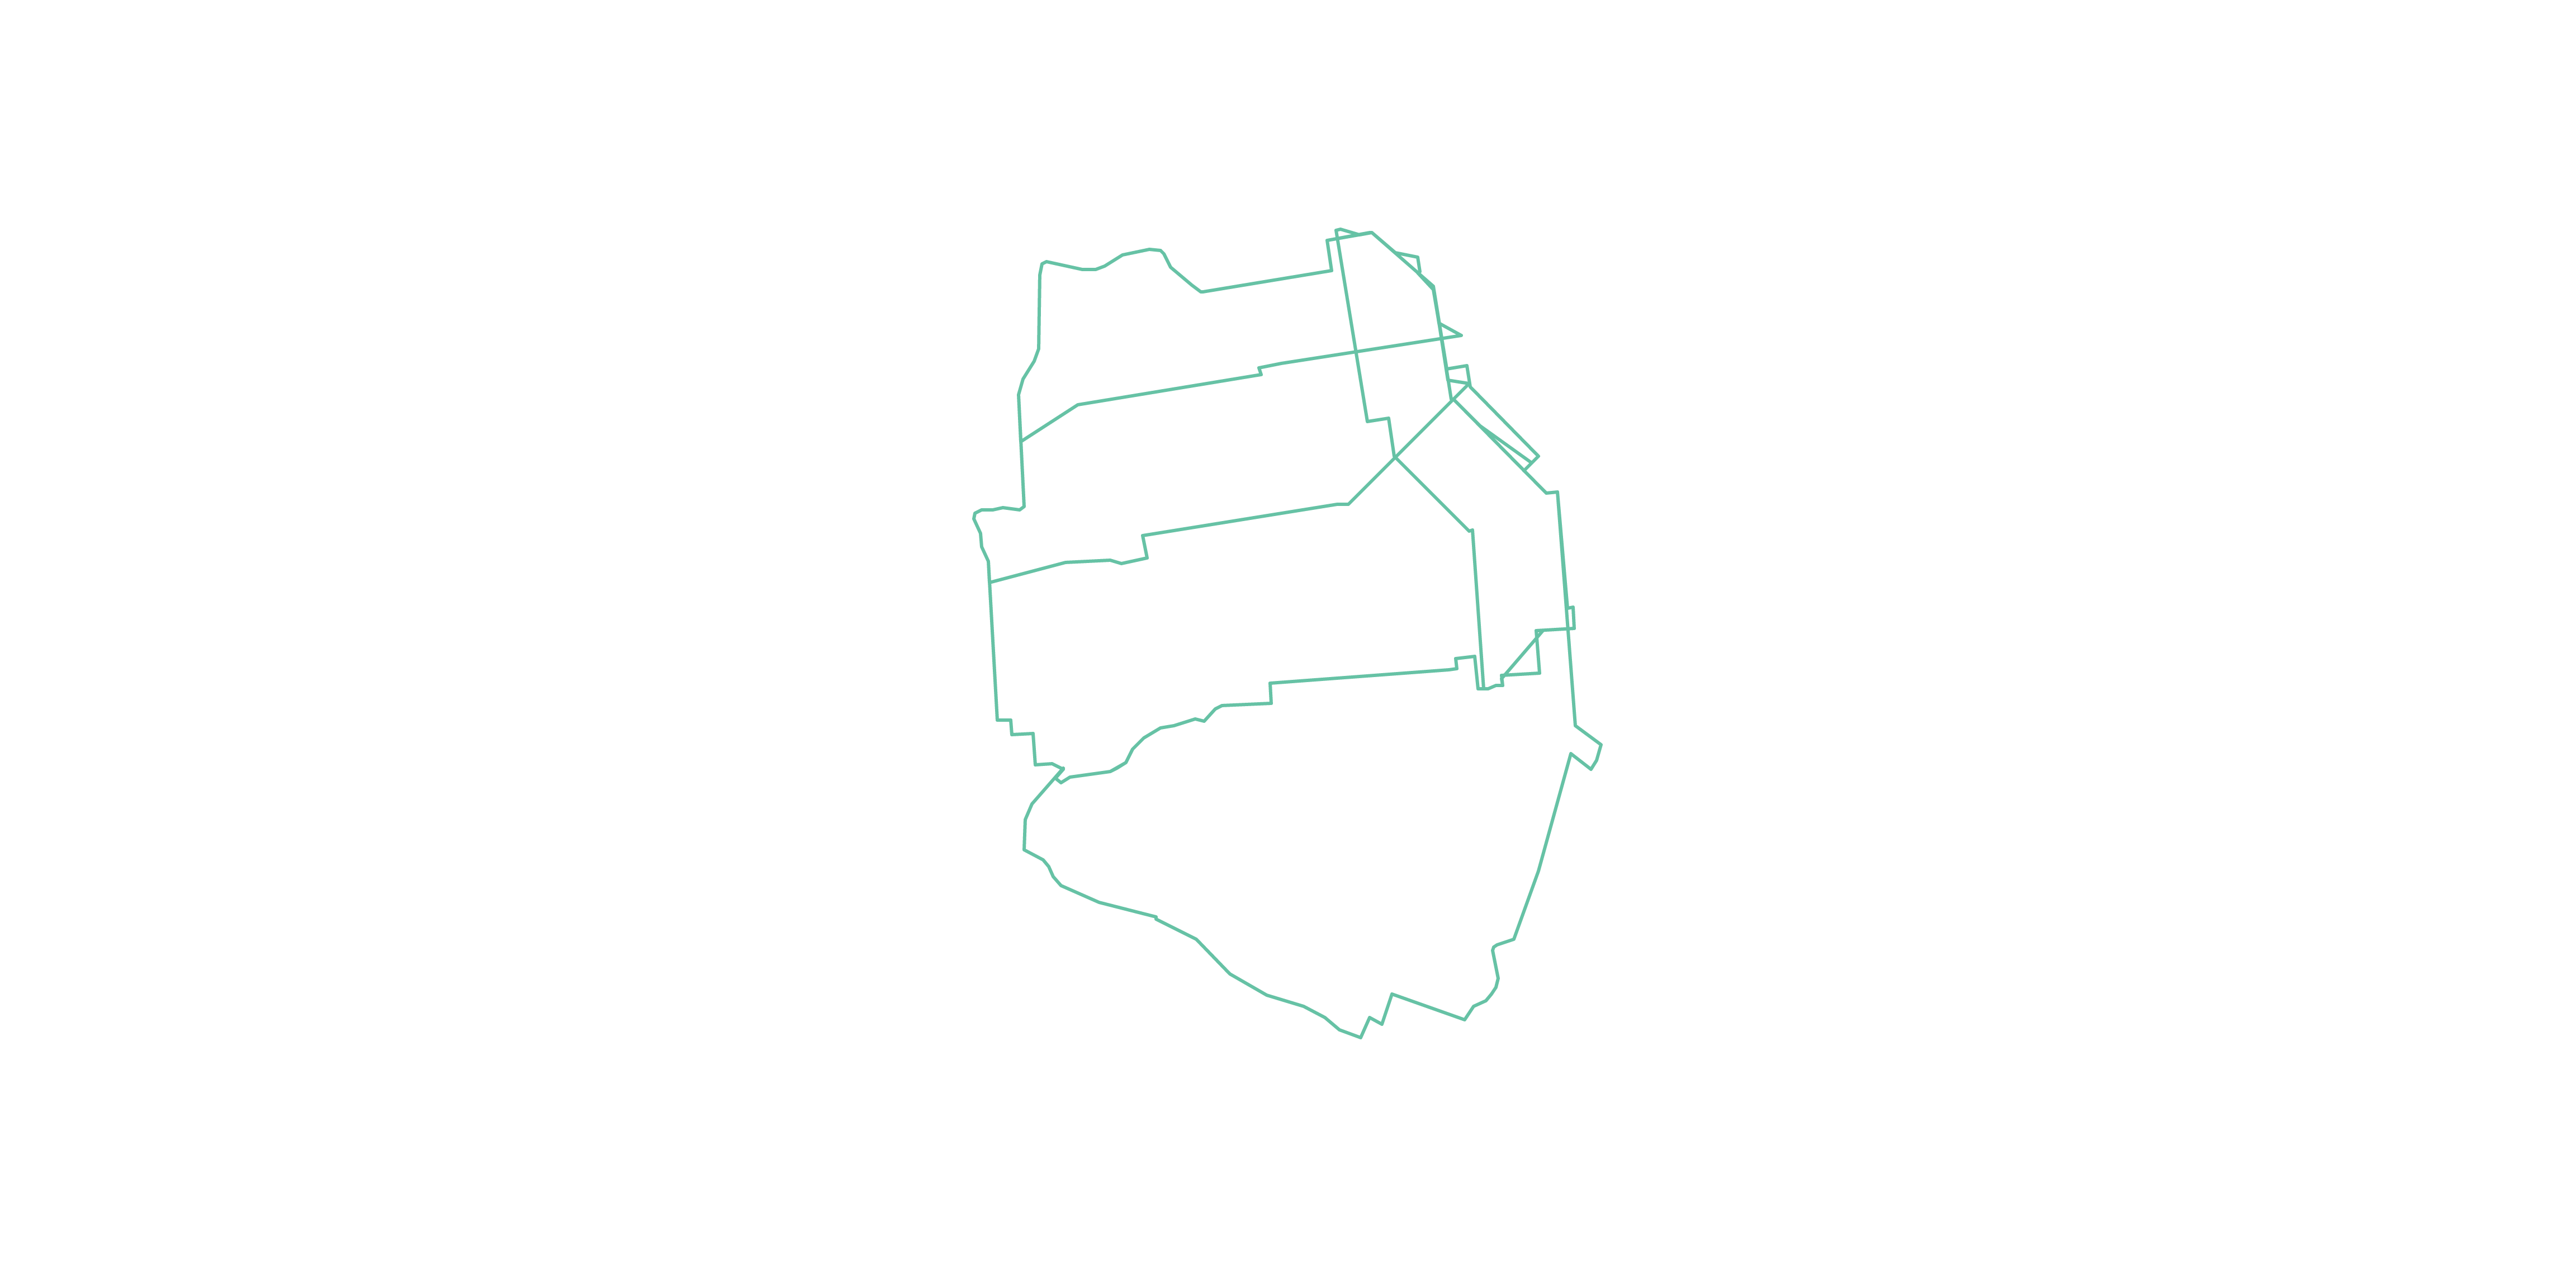
\includegraphics[width=\linewidth]{Presentation/diagrams/long_route.png}
  \caption{Example Route from best performer}\label{fig:long_route}
\endminipage
}
\begin{itemize}
    \item Fitness values \textbf{exponentially} growing. 
    \item Best performer creates \textbf{unrealistic super routes}. 
\end{itemize}
\end{figure}
\end{frame}

\section{Improved Version}

\begin{frame}{New Fitness Function and Zone Evaluator}
\begin{figure}
\minipage{0.40\textwidth}%
  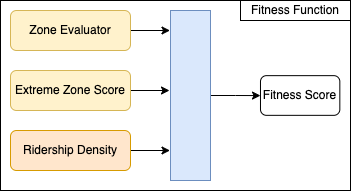
\includegraphics[width=\linewidth]{Presentation/diagrams/new-fitness-function.png}
  \caption{New Fitness Function}\label{fig:long_route}
\endminipage\hfill
\minipage{0.40\textwidth}
  \frame{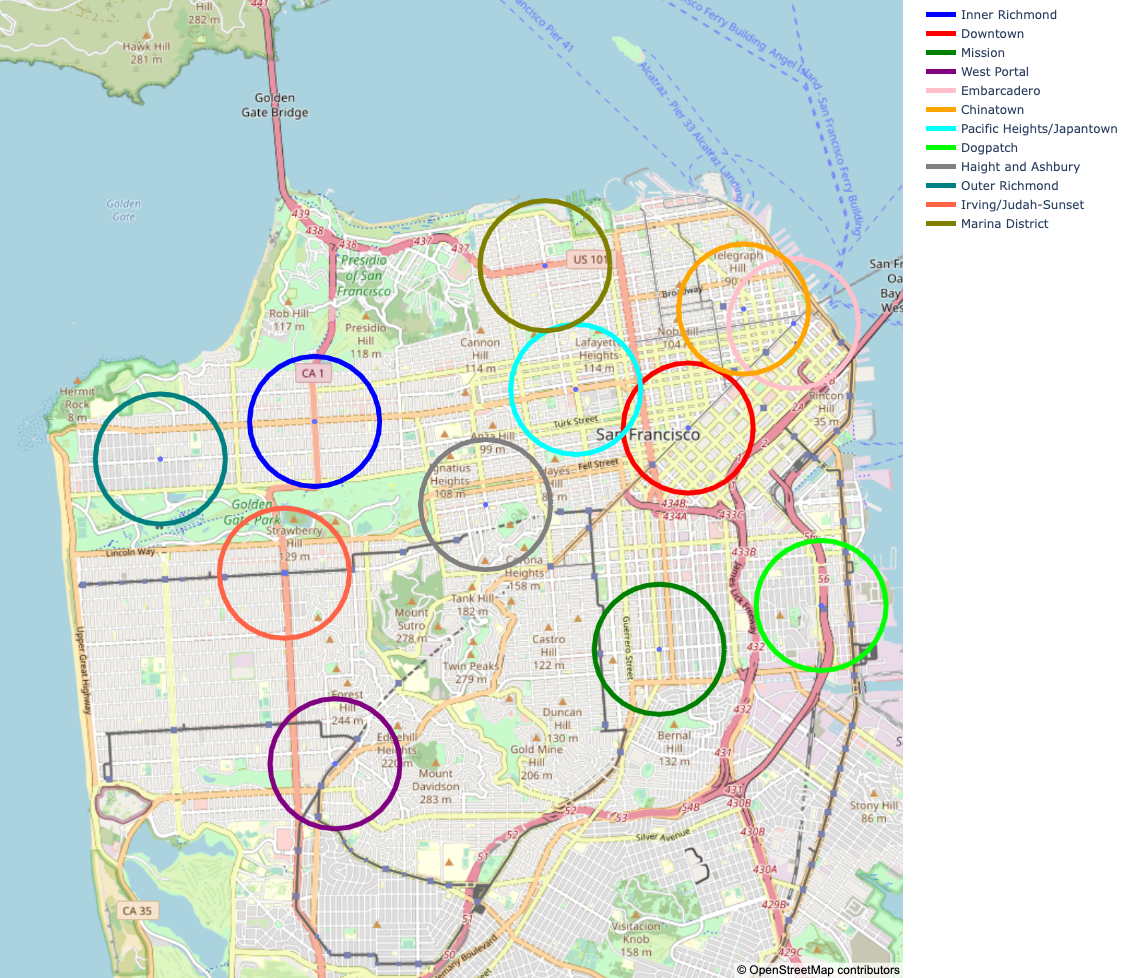
\includegraphics[width=\linewidth]{Presentation/diagrams/zone-plot.png}}
  \caption{Plot of zones}\label{fig:fitness_breakdown}
\endminipage
\begin{itemize}
    \item New \textbf{Zone Evaluator} metric.
    \item New \textbf{extreme trip} penalty. 
\end{itemize}
\end{figure}
\end{frame}

\begin{frame}{New Results}
\minipage{0.33\textwidth}
\begin{itemize}
    \item Ran \textbf{11} different hyper-parameter configurations. 
    \item Population size down to 100. 
\end{itemize}
\endminipage
\minipage{0.66\textwidth}%
\begin{figure}
  \fbox{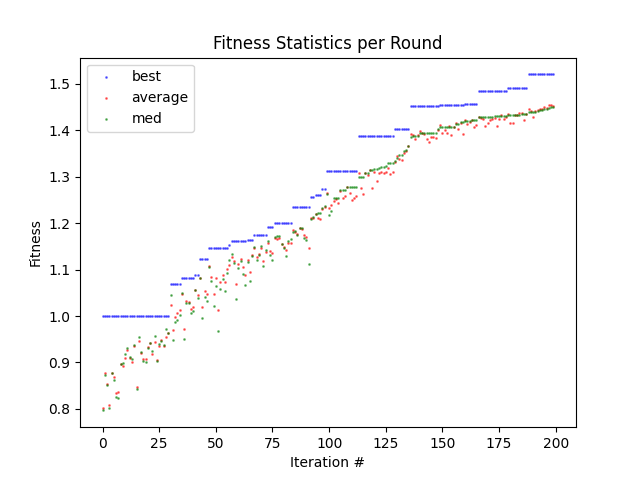
\includegraphics[width=0.55\linewidth]{Thesis/diagrams/second_run/fitness_trend(631).png}}
    \fbox{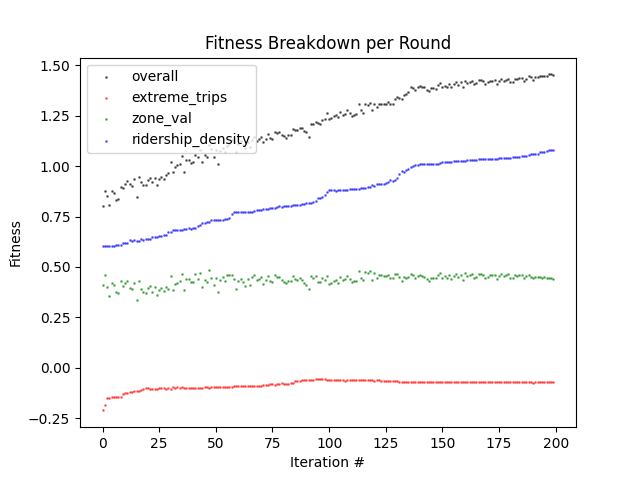
\includegraphics[width=0.55\linewidth]{Thesis/diagrams/second_run/fitness_breakdown(631).png}}
\end{figure}
\endminipage
\end{frame}



\begin{frame}{Final Results and Future Work}
\minipage{0.40\textwidth}
\begin{itemize}
    \item Bias towards downtown routes. 
    \item Lack of \textbf{genetic diversity}. 
    \item Zones are \textbf{arbitrary} at the moment.
    \item Code at \url{https://github.com/Hweinstock/Math-thesis}
\end{itemize}
\endminipage \hfill
\minipage{0.60\textwidth}%
\begin{figure}
  \fbox{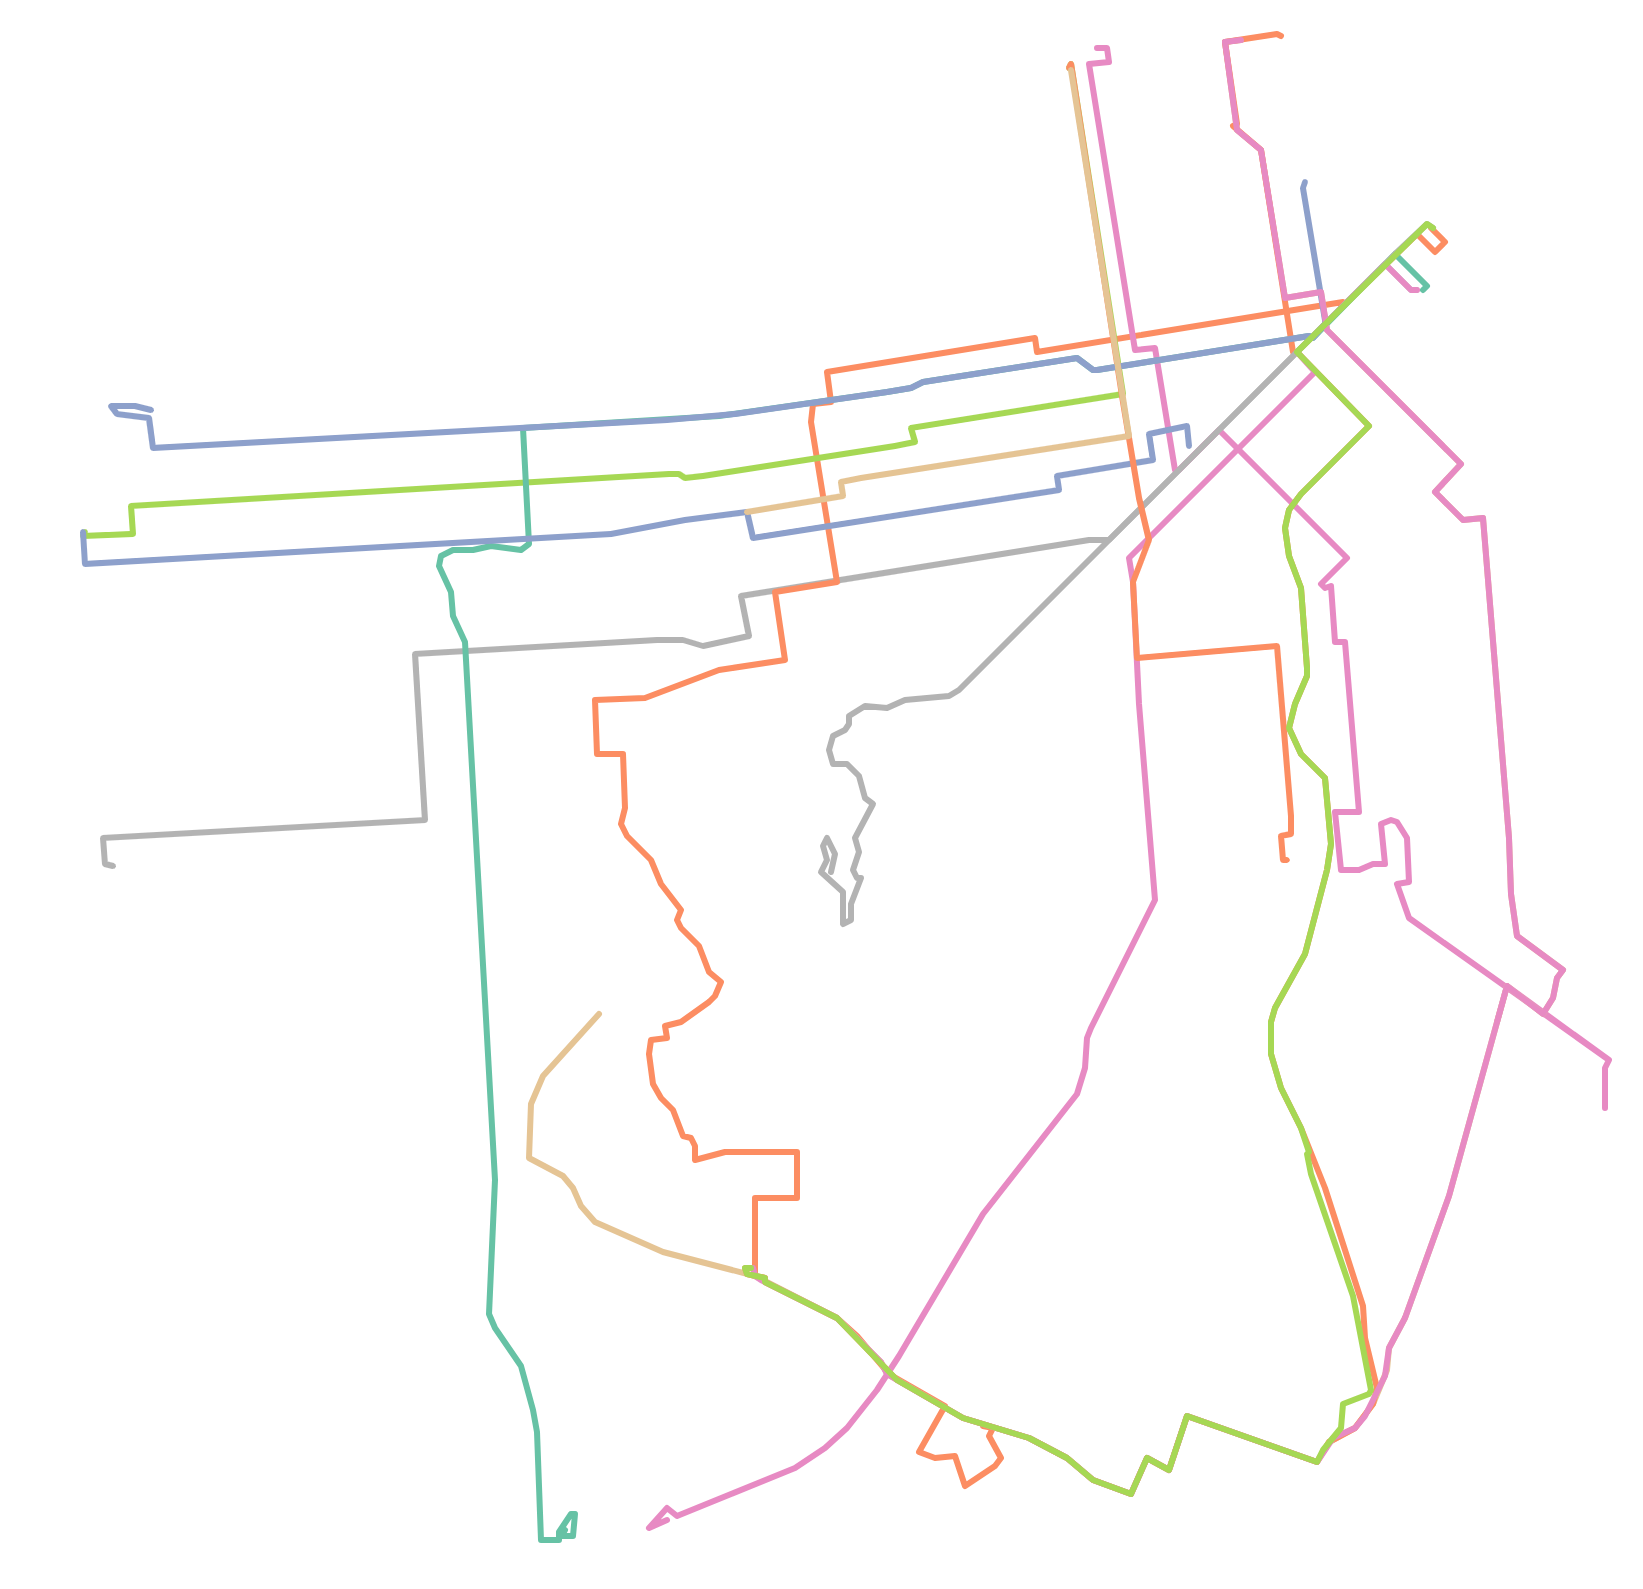
\includegraphics[width=0.75\linewidth]{Thesis/diagrams/second_run/new-downtown-routes.png}}
  \caption{SPCrossover routes in best performer}
\end{figure}

\endminipage
\end{frame}

\appendix



\begin{frame}{Bibliography}
    \printbibliography
\end{frame}

\end{document}